\clearpage
\section{Sanctuary Furnishings}
The architecture of the sanctuary directs the assembly toward two tables---the table of God's Word at the ambo and the table of Christ's Body at the altar---while reserving a noble place apart for the tabernacle and a clear visible setting for the font of Baptism.

\PCDPlateHeader{Plate II --- Principal Sanctuary Furnishings}{Not to common scale}
\ifdefined\TriptychPrintEdition
\begin{center}
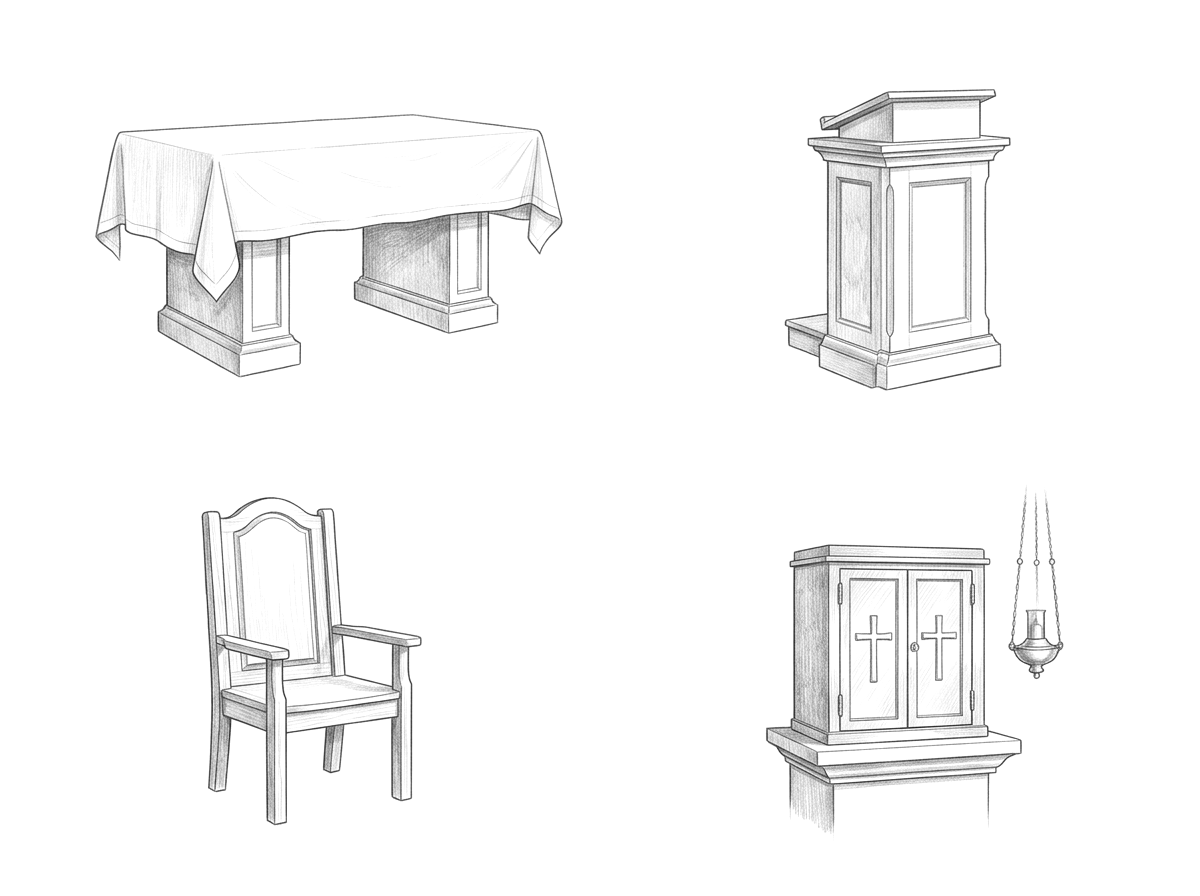
\includegraphics[width=0.92\linewidth,height=3.55in,keepaspectratio]{liturgy/roman-rite/postconciliar/2008-latin-2011-us-english/reference/roman-sanctuary-dictionary/shared/artwork/graphite/pc-art-02-altar-ambo-chair.png}
\end{center}
\PCDPositionKey{Top left: freestanding Altar covered with white linen cloth; top right: stationary stone Ambo with sloped desk and step; bottom left: dignified wooden Presidential Chair; bottom right: locked double-door Tabernacle on stone pedestal beside suspended oil Sanctuary Lamp.}
\else
\textbf{Visual Plate Summary (Plate II --- Principal Sanctuary Furnishings, Not to common scale):} Four-subject monochrome graphite architectural study comparing the principal sanctuary furnishings: top left, a freestanding carved stone altar dressed in a white linen altar cloth; top right, a permanent paneled stone ambo with angled book rest and rear step; bottom left, a stately wooden presidential chair with armrests; bottom right, a solid locked double-door metal tabernacle on a stone pedestal with a suspended sanctuary lamp burning beside it.

\textbf{Reading order and object placement:} Top left: freestanding Altar covered with white linen cloth; top right: stationary stone Ambo with sloped desk and step; bottom left: dignified wooden Presidential Chair; bottom right: locked double-door Tabernacle on stone pedestal beside suspended oil Sanctuary Lamp.
\fi

\label{pc-obj-altar}
\PCDEntryHead{Altar}{Altare}{required}{N01}
\PCDField{Also called}{Altar Table; Mensa; \textit{Mensa Domini}; \textit{Altare fixum}; \textit{Altare mobile}}
The altar is the sacred table at the heart of the sanctuary upon which the Sacrifice of the Cross is made present under sacramental signs and the people of God gather for the Eucharistic banquet. Shown in Plate II as a freestanding rectangular stone table resting on twin paneled pedestals with molded plinths and dressed smoothly in an overhanging white linen cloth, and in Plate I centered in the sanctuary with two lighted candles and a crucifix---free of gradines, altar cards, or an attached rail.

\PCDField{Plate position and status}{Top left (Plate II); center (Plate I) (Universal Roman law)}
\PCDField{Placement and liturgical use}{Universal Roman law recommends a single fixed altar in newly built churches, set apart from the rear wall so ministers may walk around it and celebrate Mass facing the people wherever possible (GIRM 299, 303), while the Holy See clarified on 25 September 2000 (Prot. N. 2036/00/L) that this expresses pastoral desirability rather than a juridical ban on historical wall-attached altars or celebration facing the apse. A fixed altar is solemnly dedicated by the bishop (GIRM 300; CIC can. 1235), with relics of saints fittingly placed beneath it rather than recessed into the mensa (GIRM 302). From the start of Mass until the Preparation of the Gifts, only the Book of the Gospels rests upon the dressed mensa; during the Liturgy of the Eucharist, only the corporal, sacred vessels, Roman Missal, and necessary items appear there (GIRM 306).}
\PCDField{United States norm}{In the Dioceses of the United States of America, the Bishops' Conference adaptation to GIRM 301 permits a fixed altar table to be crafted from dignified, solid, well-worked wood rather than natural stone, provided the structure remains permanently immovable; United States GIRM 304 likewise allows festive colored cloths beneath the required white uppermost cloth.}
\PCDField{Ministers and server boundary}{Ordinary ministers: Bishop, Priest, Deacon. Server recognizes only; does not handle: Servers venerate the altar with a profound bow on approaching or departing (genuflecting instead if the Blessed Sacrament is reserved in the sanctuary), place the Roman Missal and unconsecrated vessels upon it at the Preparation of the Gifts when needed, and never lean upon, clutter, or kiss the mensa (kissing the altar belongs to the bishop, priest, and deacon).}
\PCDSafety{Keep the altar table clear of spare papers, cruets, and extraneous items (GIRM 306), guard against candle flames and dripping wax near the white cloth, and notify the priest or deacon immediately if any Precious Blood is spilled---never attempt to blot or wash a spill yourself (GIRM 280).}
\PCDField{Distinguish from}{Credence Table}
\PCDField{Symbolism}{The Church reveres the altar as the sign of Christ Himself---both Priest and Victim---and as the table of the Lord where the Sacrifice of the Cross is made present under sacramental signs. A fixed stone altar permanently signifies Christ the Living Stone, recalling 1 Pet 2:4 (``Unto whom coming, as to a living stone, rejected indeed by men but chosen and made honourable by God:''), 1 Cor 10:4 (``and the rock was Christ.''), and Heb 13:10 (``We have an altar whereof they have no power to eat who serve the tabernacle.''). St. Thomas Aquinas similarly teaches that the altar signifies Christ Himself and, when made of stone, calls to mind both Christ the Rock and the stone sepulchre in which His body rested. (GIRM 296, 298; 1 Pet 2:4; 1 Cor 10:4; Heb 13:10; St. Thomas Aquinas, Summa Theologiae III, q. 83, a. 3)}
\PCDField{1962 Roman Missal counterpart}{\PCDTag{materially changed} Whereas the 1962 Roman Missal ordinarily presupposed a stone altar (or recessed consecrated altar stone holding relics inside the mensa) dressed with three cloths, candlesticks, central crucifix, three altar cards, and normally the tabernacle, the 2008/2011 Missal recommends a single freestanding altar wherever possible (GIRM 299, 303), deposits saints' relics beneath the altar (GIRM 302), clears the mensa of altar cards and extraneous items (GIRM 306), and in the United States permits solid wood for a fixed altar mensa (US GIRM 301).}
\PCDEntryRule

\label{pc-obj-ambo}
\PCDEntryHead{Ambo}{Ambo}{required}{N02}
\PCDField{Also called}{Lectern of the Word; \textit{Lectrinum}}
The ambo is the stationary architectural stand in the sanctuary reserved exclusively for proclaiming the Word of God during the liturgy. Depicted in Plate II as a permanent paneled stone structure resting on a molded base with a rear minister's step and an inclined book desk sized for the Lectionary or Book of the Gospels, and placed in the left foreground of Plate I in clear visual harmony with the freestanding altar.

\PCDField{Plate position and status}{Top right (Plate II); left foreground (Plate I) (Universal Roman law)}
\PCDField{Placement and liturgical use}{Universal Roman law prescribes a permanent, stationary ambo---never a lightweight movable lectern---positioned so that the attention of the faithful turns naturally toward it during the Liturgy of the Word and ministers can be clearly seen and heard (GIRM 309; Ordo lectionum Missae 32--34). Only the Scripture readings, the Responsorial Psalm, and the Easter Proclamation (Exsultet) are proclaimed from the ambo, together with the homily and the intentions of the Universal Prayer; parish announcements, commentary, and the leading of general singing belong at a separate stand elsewhere.}
\PCDField{Ministers and server boundary}{Ordinary ministers: Bishop, Priest, Deacon, Instituted lector. Server recognizes only; does not handle: Servers flank the ambo with lighted candles and incense during the Gospel proclamation and may confirm before Mass that the Lectionary rests open upon the desk, but never proclaim readings or lead prayers from the ambo unless separately deputed as readers.}
\PCDSafety{Watch the rear step of the ambo when moving into place with lighted Gospel candles or a smoking thurible, keeping flames well clear of the microphone, Lectionary pages, and ministers' vestments.}
\PCDField{Distinguish from}{Missal Stand}
\PCDField{Symbolism}{The General Instruction pairs the ambo with the altar as the two tables of the Mass---the table of God's Word and the table of Christ's Body---directing that the dignity of Sacred Scripture be honored by a fixed, noble place toward which the congregation naturally turns. Its prominence visibly echoes the Psalmist's confession in Ps 118:105 [Heb 119:105]: ``Thy word is a lamp to my feet, and a light to my paths.'' (GIRM 28, 309; Ordo lectionum Missae (1981) Praenotanda 32--34; Ps 118:105 [Heb 119:105])}
\PCDField{1962 Roman Missal counterpart}{\PCDTag{newly provided} The 1962 Roman Missal did not prescribe a permanent sanctuary ambo: at Low Mass the priest read the Epistle and Gospel from opposite corners of the altar, and at Solemn Mass the subdeacon and deacon sang them from the sanctuary floor with the subdeacon holding the Gospel book (RS VI.4--5). Postconciliar law restores a dedicated stationary ambo as a standard architectural appointment of every sanctuary (Inter Oecumenici 96; GIRM 309).}
\PCDEntryRule

\label{pc-obj-presidential-chair}
\PCDEntryHead{Presidential Chair}{Sedes sacerdotis celebrantis}{required}{N03}
\PCDField{Also called}{Chair for the Priest Celebrant; Presider's Chair; \textit{Sedes}}
The presidential chair is the single seat appointed for the priest celebrant from which he presides over the liturgical assembly and leads its opening and closing prayers. Shown at bottom left of Plate II as a dignified wooden armchair with an arched paneled high backrest, sturdy armrests, and squared legs, and positioned at rear right in Plate I beside the credence table---clearly superior to server seating yet deliberately devoid of canopy, royal steps, or throne-like ornament.

\PCDField{Plate position and status}{Bottom left (Plate II); rear right (Plate I) (Universal Roman law)}
\PCDField{Placement and liturgical use}{Under universal Roman law, the chair is best set at the head of the sanctuary facing the congregation unless architectural distance or a centrally placed tabernacle behind the altar makes another clear position more suitable (GIRM 310). From this seat the priest conducts the Introductory Rites (including the Collect), listens to the Scripture readings and may preach the homily, leads the Universal Prayer, and concludes Mass with the Prayer after Communion and dismissal (GIRM 124, 127--130, 165--167). The Roman Missal---or, in the United States, the lighter Book of the Chair---and any needed hymnal are prepared beside it (GIRM 118a). In a cathedral church, the diocesan bishop presides from his permanent cathedra rather than a presbyteral chair (Caeremoniale Episcoporum 1984).}
\PCDField{Ministers and server boundary}{Ordinary ministers: Priest, Bishop. Clergy-reserved; server does not touch: Reserved strictly to the priest celebrant (or bishop when celebrating outside his cathedral); altar servers never sit in the presidential chair and approach it solely to hold the Roman Missal or Book of the Chair during prayers.}
\PCDField{Symbolism}{The General Instruction assigns the presidential chair a clear functional sign value: it manifests the priest celebrant's office of presiding over the gathered assembly and directing its prayer, while explicitly excluding any likeness to a royal throne. (GIRM 310)}
\PCDField{1962 Roman Missal counterpart}{\PCDTag{materially changed} In the 1962 Roman Rite, presbyteral seating consisted of a three-seat bench (sedilia) placed along the Epistle side of the sanctuary solely for sitting during sung chants and lessons while all orations were spoken at the altar. Postconciliar law replaces those lateral seats with a focal single chair from which the priest leads the Introductory Rites, Liturgy of the Word, and Concluding Rites (Inter Oecumenici 92; GIRM 310).}
\PCDEntryRule

\label{pc-obj-credence-table}
\PCDEntryHead{Credence Table}{Abacus}{required}{N04}
\PCDField{Also called}{Side Table; Credence; \textit{Credentia}; \textit{Mensa credentiae}}
The credence table is the side table set in a convenient corner of the sanctuary to hold sacred vessels, altar linens, cruets, and lavabo articles off the altar until they are needed. Shown at the far right of Plate I beside the presidential chair as a compact, four-legged rectangular wooden side table with a lower shelf, carrying the paired glass cruets on their tray and folded white linens neatly stacked below.

\PCDField{Plate position and status}{See Plate I, far right beside the presidential chair (Universal Roman law)}
\PCDField{Placement and liturgical use}{GIRM 118c appoints the credence table (abacus) as the preparation station for every Mass with a congregation, holding the chalice, folded corporal, purificator, optional pall and chalice veil, paten, ciboria, bread and wine cruets (unless carried in the Procession of Gifts), vessel of blessed water for the Sunday sprinkling rite, Communion-plate, and lavabo pitcher, basin, and towel. Keeping these items on the credence table preserves an uncluttered altar mensa until the Preparation of the Gifts (GIRM 139, 306). After Communion or immediately after Mass, sacred vessels may also be purified at the credence table by a priest, deacon, or instituted acolyte (GIRM 279).}
\PCDField{Ministers and server boundary}{Ordinary ministers: Priest, Deacon, Instituted acolyte. Server prepares or sets in place before or during Mass: Servers help arrange clean unconsecrated vessels, linens, cruets, and lavabo equipment on the credence table before Mass, carry needed items to the altar at the Preparation of the Gifts, and bring the water cruet for purification without touching unpurified sacred vessels.}
\PCDSafety{After Communion, never purify sacred vessels at the credence table and never disturb unpurified vessels left suitably covered upon a corporal there; purification belongs strictly to the priest, deacon, or instituted acolyte (GIRM 279; Redemptionis Sacramentum 119; USCCB Norms 53).}
\PCDField{Distinguish from}{Altar}
\PCDField{1962 Roman Missal counterpart}{\PCDTag{continued} Both the 1962 Roman Missal (RG 528; RS II.5) and the 2008/2011 GIRM (118c, 139, 279) appoint a sanctuary side table (abacus) for cruets, lavabo articles, Communion-plate, and vessels. In postconciliar Mass with a congregation, its role expands because the chalice and linens also ordinarily wait there until the Preparation of the Gifts (rather than being carried to the altar by the priest at the start of Low Mass) and vessel purification commonly takes place at the credence table (GIRM 279).}
\PCDEntryRule

\label{pc-obj-tabernacle}
\PCDEntryHead{Tabernacle}{Tabernaculum}{required}{N05}
\PCDField{Also called}{Eucharistic Tabernacle}
The tabernacle is the immovable, solid, locked sacred shrine in which the Most Holy Eucharist is reserved for Viaticum, Communion of the sick, and the adoration of the faithful. Illustrated at bottom right of Plate II as a rectangular solid metal safe with lockable double doors bearing relief crosses anchored upon a stone pedestal, and in Plate I as a domed opaque metal tabernacle set atop a pillar inside a recessed arched niche at the rear of the sanctuary, accompanied in both views by a hanging sanctuary lamp.

\PCDField{Plate position and status}{Bottom right (Plate II); recessed rear niche (Plate I) (Universal Roman law)}
\PCDField{Placement and liturgical use}{Universal Roman law requires ordinarily one tabernacle in a church or oratory, immovable, crafted of solid opaque material, securely locked against danger of profanation, and blessed before liturgical use (GIRM 314; CIC can. 938; Redemptionis Sacramentum 130). Because the sign of Mass is clearer when the tabernacle does not stand upon the altar of celebration, universal law (GIRM 315) entrusts the Diocesan Bishop to place it either in the sanctuary apart from the altar of celebration---not excluding a former high altar no longer used for Mass---or in a distinct chapel suitable for private adoration that is organically connected to the church and readily visible to the faithful. The pastor or rector must diligently safeguard the tabernacle key (CIC can. 938 §5).}
\PCDField{Ministers and server boundary}{Ordinary ministers: Bishop, Priest, Deacon. Clergy-reserved; server does not touch: Strictly reserved to clergy (and to instituted acolytes or duly deputed extraordinary ministers solely for Communion distribution or reposition); altar servers never open the tabernacle, handle its key, or touch reserved vessels, and genuflect before it outside Mass and at the beginning and end of Mass when it stands in the sanctuary (GIRM 274).}
\PCDSafety{Never open the tabernacle, touch the tabernacle key, or retrieve or repose the Blessed Sacrament. Key custody belongs strictly to the pastor or rector (CIC can. 938 §5). Genuflect on the right knee before the tabernacle outside Mass and at the beginning and end of Mass when it stands in the sanctuary (GIRM 274).}
\PCDField{Symbolism}{The Church honors the tabernacle as the consecrated dwelling of Christ's abiding sacramental presence in the midst of His people, recalling the Lord's promise to Israel in Ex 25:8 (``And they shall make me a sanctuary, and I will dwell in the midst of them:''). Setting the tabernacle apart from the altar of celebration keeps distinct the sign of Christ's reserved presence for adoration and Viaticum from the sacrificial action of Mass, fulfilling the constant pastoral care that St. Thomas Aquinas grounds in bringing the Eucharist to the sick without delay. (GIRM 314--315; Eucharisticum Mysterium (1967) 53--55; Ex 25:8; St. Thomas Aquinas, Summa Theologiae III, q. 83, a. 5, ad 11)}
\PCDField{1962 Roman Missal counterpart}{\PCDTag{materially changed} Both the 1917 Code (cann. 1268--1269) and current law (CIC 1983 can. 938; GIRM 314) mandate a single immovable, solid, opaque, securely locked tabernacle. Whereas 1917/1962 discipline ordinarily fixed the veiled tabernacle in the middle of the high altar of celebration, GIRM 315 considers it clearer as a sign not to place it on the altar where Mass is celebrated, entrusting the Diocesan Bishop to choose either another worthy place in the sanctuary or an organically connected adoration chapel, and no longer universally mandating a tabernacle veil.}
\PCDEntryRule

\label{pc-obj-sanctuary-lamp}
\PCDEntryHead{Sanctuary Lamp}{Lampas peculiaris}{required}{N06}
\PCDField{Also called}{Tabernacle Lamp; Presence Lamp; \textit{Lampas sanctuarii}; \textit{Lucerna}}
The sanctuary lamp is the dedicated oil or wax lamp kept burning continuously near the tabernacle to announce and honor the Eucharistic presence of Christ. Shown at bottom right of Plate II and beside the recessed rear niche in Plate I as a rounded metal lamp bowl suspended on three chains from a ceiling mount or wall bracket, cradling a cylindrical glass globe (traditionally red or clear) that shields a living oil or beeswax flame.

\PCDField{Plate position and status}{Suspended beside the tabernacle at bottom right (Plate II) and in the rear niche (Plate I) (Universal Roman law)}
\PCDField{Placement and liturgical use}{Universal Roman law and canon law require a special lamp, nourished by oil or wax rather than an electric bulb, to shine permanently day and night beside every tabernacle in which the Most Holy Eucharist is reserved (GIRM 316; CIC can. 940). It is extinguished only when the tabernacle is completely emptied of the Blessed Sacrament, notably from the Mass of the Lord's Supper on Holy Thursday evening until reservation resumes at the Easter Vigil.}
\PCDField{Ministers and server boundary}{Ordinary ministers: Priest, Sacristan. Server recognizes only; does not handle: Servers look to the burning sanctuary lamp as the unmistakable sign that Christ is reserved in the tabernacle and never light, move, or extinguish it during Mass; any maintenance outside Mass follows sacristan direction with fire-safety care.}
\PCDSafety{Never extinguish, move, or adjust the sanctuary lamp during Mass, and never extinguish it while the Blessed Sacrament remains reserved in the tabernacle. If assisting the sacristan outside Mass to replace a sanctuary candle or oil vessel, allow hot glass and oil to cool safely, guard against open flame, and never open the tabernacle.}
\PCDField{Distinguish from}{Altar Candles}
\PCDField{Symbolism}{The continuously burning oil or wax lamp openly signals Christ's abiding sacramental presence in the tabernacle and renders silent honor to Him day and night, echoing the perpetual lamp commanded before the Old Covenant sanctuary in Ex 27:20--21 (``Command the children of Israel that they bring thee the purest oil of the olives, and beaten with a pestle: that a lamp may burn always, In the tabernacle of the testimony, without the veil that hangs before the testimony'') and Lev 24:2--3 (``to furnish the lamps continually, Without the veil of the testimony in the tabernacle of the covenant''). (GIRM 316; CIC (1983) can. 940; Ex 27:20--21; Lev 24:2--3)}
\PCDField{1962 Roman Missal counterpart}{\PCDTag{continued} Postconciliar discipline continues the 1917/1962 requirement without interruption: both CIC (1917) can. 1271 and CIC (1983) can. 940 together with GIRM 316 require a special living flame of oil or wax to burn continually before or near the tabernacle whenever the Eucharist is reserved.}
\PCDEntryRule

\label{pc-obj-baptismal-font}
\PCDEntryHead{Baptismal Font}{Fons baptismalis}{required}{N07}
\PCDField{Also called}{Font; \textit{Fons baptismatis}}
The baptismal font is the permanent stone or metal water basin required in every parish church for administering the Sacrament of Baptism. Illustrated at bottom right of Plate X as a carved octagonal stone basin decorated with foliate relief panels, raised on a matching paneled pedestal and stepped plinth, with a ribbed domed cover resting ajar to expose the smooth interior basin.

\PCDField{Plate position and status}{See Plate X, bottom right (Universal Roman law)}
\PCDField{Placement and liturgical use}{The baptismal font is governed by universal canon law (CIC can. 858 §1, requiring a font in every parish church), the Rite of Baptism for Children (General Introduction 25, 45--47), and the Easter Vigil rubrics of the Roman Missal. Local architecture places it either in a distinct baptistery or in a prominent, clearly visible area near the church entrance or sanctuary so the assembly can participate in Baptisms and process to the font at the Easter Vigil; its design accommodates clean flowing or poured water (and, where provided, immersion). Bishops, priests, and deacons are the ordinary ministers of Baptism (CIC can. 861 §1).}
\PCDField{Ministers and server boundary}{Ordinary ministers: Bishop, Priest, Deacon. Server recognizes only; does not handle: Servers walk in procession to the font with cross, candles, ritual book, or drying towels during Baptisms and the Easter Vigil, never pouring sacramental water or disposing of blessed baptismal water improperly.}
\PCDSafety{Never empty blessed baptismal water into an ordinary sink or sewer drain; blessed water must be poured reverently into the sacrarium or directly into clean earth. Wipe any splashed water from stone or tiled steps immediately to prevent slipping.}
\PCDField{Distinguish from}{Aspergillum and Aspersorium}
\PCDField{Symbolism}{The ancient Roman Easter Vigil blessing calls the baptismal font the motherly womb from which the Church brings forth new children in Christ, uniting the Lord's teaching in John 3:5 (``unless a man be born again of water and the Holy Ghost, he cannot enter into the kingdom of God.'') with St. Paul's mystery of death and resurrection in Rom 6:3--4 (``Know you not that all we who are baptized in Christ Jesus are baptized in his death? For we are buried together with him by baptism into death: that, as Christ is risen from the dead by the glory of the Father, so we also may walk in newness of life.''). Early Christian catechesis, including St. Cyril of Jerusalem, expounds the font as both tomb and womb of new creation, reflected architecturally in the classic octagonal basin of the eighth day. (Roman Missal Easter Vigil; CCC 1237--1243; John 3:5; Rom 6:3--4; St. Cyril of Jerusalem, Mystagogical Catechesis 2.4)}
\PCDField{1962 Roman Missal counterpart}{\PCDTag{materially changed} Both 1962 discipline and CIC (1983) can. 858 require a baptismal font in every parish church. Whereas 1962 practice ordinarily enclosed the font inside a gated baptistery near the church entrance and blessed the year's water at the Easter Vigil with an infusion of Oil of Catechumens and Sacred Chrism directly into the basin, postconciliar rites bless fresh water at each Baptism outside Easter Time without pouring oils into the font and favor congregationally visible placement suited to pouring or immersion.}
\PCDEntryRule
